% Introducción a los tres enfoques y enfatizar el trabajo a mano por Freeman. 
\noindent
Bajo un enfoque \emph{clásico}, existen tres formas de mejorar la resolución 
de una imagen:

\begin{itemize}
    \item Amplificación de detalles existentes
    \item Suma de múltiples frames
    \item Único frame
\end{itemize}

Para el primero de ellos, se realiza una amplificación de las frecuencias altas
(donde se encuentran los detalles existentes de la imagen) dada la variación local
entre los pixeles vecinos. 
La amplificación de detalles existentes resulta bastante 
sencillo de aplicar. Sin embargo, ante imágenes con una cantidad considerable de
ruido puede no ser la mejor opción a tomar. Además, al potencializar las 
frecuencias ya existentes de la imagen, el resultado estará definido por el detalle
previo en la imagen de entrada. 

El segundo de los métodos considera que el frame de alta resolución es el resultado
de una secuencia de frames de baja resolución que permiten obtener las frecuencias 
altas de la imagen resultante para mejorar su resolución. Esto es conveniente cuando
ya se cuenta con el conjunto de imágenes requeridas y se planea realizar una 
reconstrucción de la imagen en una mejor resolución.

Por otro lado, el tercer método basado en un único frame o imagen busca aproximar las
frecuencias altas (detalles) que no se encuentra en la entrada del algoritmo y que evidentemente
no puede obtenerse sólo amplificando las frecuencias altas como lo que ocurre con 
el primero de los métodos. 

\subsection{Interpolación}
\noindent
Para mejorar la resolución se busca aumentar la densidad de pixeles de la imagen con el objetivo
de hacer la imagen más grande y mejorar sus detalles a partir de la predicción de 
pixeles que no se encuentran en la imagen visiblemente, pero que podrían aproximarse
al buscar que se mantenga una consistencia en la imagen modificada de acuerdo a la
vecindad de los pixeles. 

Esto permite proponer el uso de algoritmos de interpolación que buscan predecir los  3
pixeles vecinos y con ello aumentar la densidad de pixeles de la imagen de entrada. 
Con base en \cite{interpolation_cambridge}, dichos algoritmos pueden agruparse en dos
categorías: adaptativos y no adaptativos. Los primeros cambian dependiendo de lo que
se está interpolando (bordes o texturas suaves) pixel por pixel con el objetivo de
minimizar los errores antiestéticos de los algoritmos de interpolación como el
desenfoque o pérdida de detalles en regiones evidentes. Ejemplos de ellos pueden
ser los softwares de licencia como \emph{Qimage, PhotoZoom Pro, Genuine Fractals, etc}. 

Mientras que los métodos no adaptativos tratan todos los pixeles por igual
dada la predicción de un pixel central de acuerdo a sus pixeles adyacentes. Esto 
involucra que entre más vecinos se consideren en la interpolación, una mejor 
aproximación se tendrá del pixel a predecir, pero de manera proporcional 
aumentarán los recursos computacionales necesarios. Dentro de los algoritmos 
se incluyen: \emph{vecino más cercano, bilineal, bicúbica, spline, entre otros.}

A continuación se describirán algunos de los algoritmos no adaptativos para 
interpolación que serán utilizados en los diferentes métodos para \emph{Súper
Resolución}:
\begin{itemize}
    \item \textbf{Vecino más cercano} - Dado un pixel considera sólo un pixel 
    adyacente para la interpolación, lo que resulta en un menor tiempo de procesamiento
    pero resultados poco consistentes al observar al conjunto de pixeles interpolados. 
    \item \textbf{Bilineal} - Considera una vecindad 2x2 correspondiente al pixel
    a predecir con su correspondiente promedio ponderado de acuerdo a la distancia
    del pixel desconocido. Esto da como resultado un aspecto más suave que el vecino
    más cercano. 
    \item \textbf{Bicúbica} - Valora una vecindad 4x4 de pixeles conocidos para la
    predicción del pixel central considerando el mismo procedimiento de la 
    interpolación bilineal. Como resultado, se alcanzan imágenes más nítidas que los 
    métodos anteriores. Logrando así un equilibrio entre la resolución de salida y el 
    tiempo de procesamiento. Lo anterior promueve que sea un estándar en muchos programas
    de edición de imágenes, controladores de impresoras e interpolación en cámaras. 
\end{itemize}

En la Figura \ref{fig:interpoladores} se presentan los tres algoritmos no adaptativos
más utilizados. Observe que las definiciones dadas anteriormente coinciden con los 
resultados expuestos donde el \emph{vecino más cercano} resulta poco útil para
predecir los pixeles intermedios mientras que \emph{bilineal} o \emph{bicúbica}
predicen de mejor manera los pixeles intermedios con un poco más de detalle para
en el caso del último algoritmo. 
 
\begin{figure}[H]
    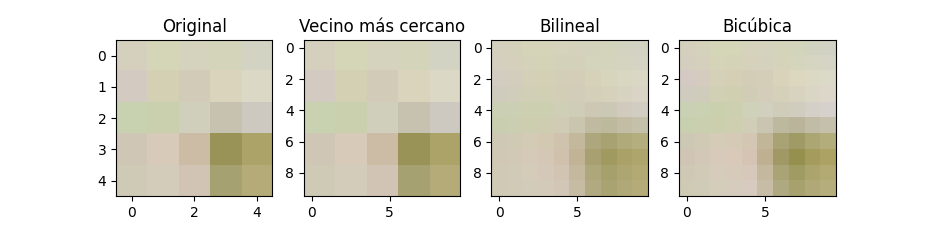
\includegraphics[scale = 0.6 ]{ tipos_interpoladores.png }
    \centering
    \caption{ Algoritmos de interpolación no adaptativos }
    \label{fig:interpoladores}
\end{figure}
Todos los interpoladores no adaptativos intentan encontrar un equilibrio óptimo
entre tres efectos no deseados: halos de borde, desenfoque y \emph{aliasing}. En la 
Figura \ref{fig:efectos_inter} puede observarse el efecto para cada caso. 

\begin{figure}[H]
    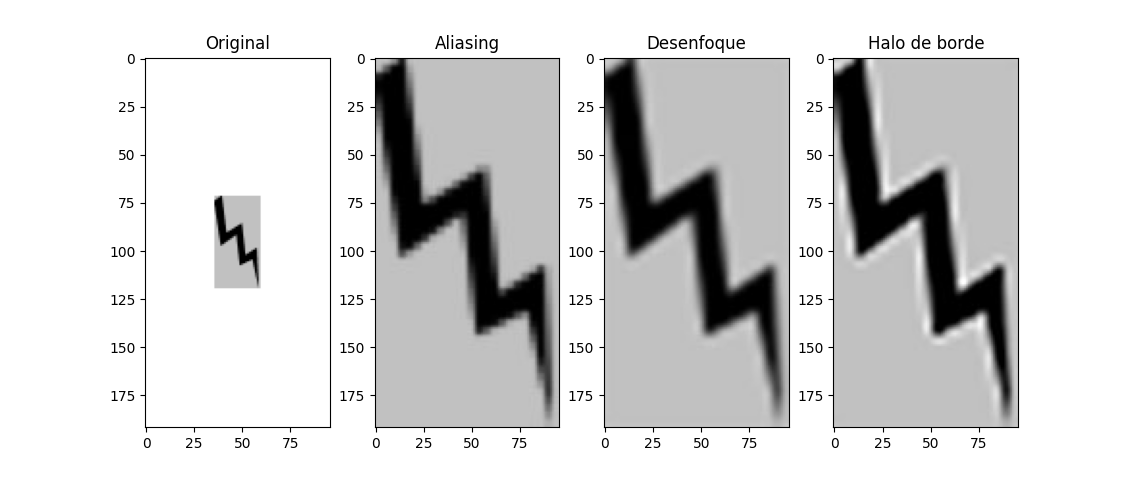
\includegraphics[scale = 0.5 ]{ efectos_inter.png }
    \centering
    \caption{ Efectos de interpolación}
    \label{fig:efectos_inter}
\end{figure}

Incluso los interpoladores no adaptativos más avanzados siempre tienden a aumentar
o disminuir algunos de los efectos a expensas de los otros dos, por lo tanto uno 
será más evidente. 

En contraste, los interpoladores adaptativos pueden o no producir los efectos 
mencionados aunque generalmente inducen texturas que no son de la imagen o 
pixeles extraños a pequeña escala.

